\documentclass[11pt]{article}

\usepackage[margin=1in]{geometry}
\usepackage{amsmath}
\usepackage{amssymb}
\usepackage{booktabs}
\usepackage{graphicx}
\usepackage{float}
\usepackage{siunitx}
\usepackage{hyperref}
\usepackage{enumitem}

\hypersetup{
  colorlinks=true,
  linkcolor=blue,
  urlcolor=blue
}

\title{Exhaustive Report: Numerical Stability of Explicit and Implicit Methods for a Bounded Memristor ODE}
\author{John Louis Lagramada \and Patrick Villareal}
\date{}

\begin{document}

\maketitle
\tableofcontents
\newpage

\section{Overview}

\subsection{Purpose of this report}

This report explains the project from the ground up. It is written for a reader who may not know what a memristor is, what a hysteresis loop means, or why numerical methods are needed for ordinary differential equations. The goal is to make the simulation, the formulas, the plots, and the conclusions understandable enough for a presentation.

The project compares three numerical methods:
\begin{itemize}[noitemsep]
  \item Explicit Euler,
  \item fourth-order Runge-Kutta, usually called RK4,
  \item Implicit Euler.
\end{itemize}

These methods are used to approximate the time evolution of a memristor's internal state. The important question is not only whether the methods produce numbers, but whether those numbers stay physically meaningful.

\subsection{Main idea in one paragraph}

A memristor is an electrical device whose resistance depends on its past behavior. In this model, the device has an internal state \(w(t)\), representing how much of the device is in a low-resistance doped state. Since this state is a physical length, it must stay between \(0\) and the full device thickness \(D\). The project applies sinusoidal voltage to the device and numerically solves the resulting initial value problem. The numerical methods are compared by checking their state trajectories, their boundary violations, their voltage-current hysteresis loops, and their runtime cost.

\subsection{What the reader should look for}

There are four main outputs:
\begin{itemize}[noitemsep]
  \item The state trajectory plot shows how \(w(t)/D\) changes over time.
  \item The boundary violation plot shows whether a numerical method leaves the physical interval \(0 \leq w \leq D\).
  \item The V-I hysteresis plot shows how current responds to voltage over repeated sinusoidal cycles.
  \item The runtime plot shows how much computational work each method costs per step.
\end{itemize}

\section{Background Concepts}

\subsection{What is a resistor?}

A resistor is a basic electrical component that opposes current. For an ideal linear resistor, Ohm's law says
\[
v = iR,
\]
where \(v\) is voltage, \(i\) is current, and \(R\) is resistance. If \(R\) is constant, the current is simply
\[
i = \frac{v}{R}.
\]
For a fixed resistor, the device has no memory. If the same voltage is applied at two different times, the same current is expected.

\subsection{What is a memristor?}

A memristor is different because its effective resistance depends on its internal state. The word ``memristor'' comes from memory and resistor. A memristor can be thought of as a resistor with memory: its current response depends not only on the present voltage, but also on how the device arrived at its present internal state.

In the HP TiO2 model used here, the device is treated as a thin film with two regions:
\begin{itemize}[noitemsep]
  \item a doped region with low resistance,
  \item an undoped region with high resistance.
\end{itemize}

The internal variable \(w(t)\) is the width of the doped region. The full device thickness is \(D\). Therefore:
\[
0 \leq w(t) \leq D.
\]
If \(w(t)=0\), none of the device is in the doped low-resistance state. If \(w(t)=D\), the whole device is doped. Values below \(0\) or above \(D\) are physically impossible.

\subsection{Why the state variable matters}

The memristor resistance changes as \(w(t)\) changes. The model defines the memristance as
\[
M(w) = R_{\text{on}}\frac{w}{D}
       + R_{\text{off}}\left(1-\frac{w}{D}\right).
\]
Here:
\begin{itemize}[noitemsep]
  \item \(R_{\text{on}}\) is the resistance when the device is fully doped,
  \item \(R_{\text{off}}\) is the resistance when the device is undoped,
  \item \(w/D\) is the fraction of the device that is doped.
\end{itemize}

This is a weighted average. When \(w/D\) is large, the device behaves more like the low-resistance state. When \(w/D\) is small, it behaves more like the high-resistance state.

\subsection{What is a hysteresis loop?}

A hysteresis loop appears when a system's output depends on its history. In this project, the input is voltage and the output is current. If the device had no memory and behaved like a fixed resistor, the voltage-current graph would be a single straight line. A memristor can produce a loop instead, because the current depends on the changing internal state \(w(t)\).

The project uses a sinusoidal voltage:
\[
v(t) = V_0 \sin(\omega t).
\]
As time advances, the voltage rises, falls, becomes negative, and returns. If current is plotted against voltage over this cycle, the curve can trace a loop. The loop is called pinched because an ideal memristor's V-I curve passes through the origin: when voltage is zero, current is also zero.

\subsection{Why hysteresis is useful in this project}

The hysteresis loop is a visual test of whether the simulation is physically meaningful. If the internal state is computed poorly, the current can become distorted because current is calculated from
\[
i(t,w) = \frac{v(t)}{M(w)}.
\]
If \(w\) leaves the physical interval, then the memristance is no longer physically valid. For this reason, the project stores two versions of the state:
\begin{itemize}[noitemsep]
  \item the raw numerical state, used to detect numerical overshoot,
  \item the clipped physical state, used to compute V-I plots.
\end{itemize}

\section{Mathematical Model}

\subsection{State equation}

The memristor state equation used in this project is
\[
\frac{dw}{dt}
=
\frac{\mu_v R_{\text{on}} v(t)}{D^2 M(w)}.
\]
The right-hand side tells us how fast \(w(t)\) changes at time \(t\). This change depends on the applied voltage \(v(t)\) and the current memristance \(M(w)\).

\subsection{Meaning of each parameter}

\begin{table}[H]
\centering
\begin{tabular}{lll}
\toprule
Symbol & Meaning & Default value used \\
\midrule
\(R_{\text{on}}\) & fully doped resistance & \SI{100}{\ohm} \\
\(R_{\text{off}}\) & undoped resistance & \SI{16000}{\ohm} \\
\(D\) & full device thickness & \SI{10e-9}{\meter} \\
\(\mu_v\) & ion mobility & \SI{1e-14}{\meter\squared\per\volt\per\second} \\
\(V_0\) & voltage amplitude & \SI{1}{\volt} \\
\(f\) & drive frequency & \SI{1e8}{\hertz} \\
\(w(0)\) & initial state & \(0.5D\) \\
\bottomrule
\end{tabular}
\caption{Default simulation parameters.}
\end{table}

\subsection{Why this is an initial value problem}

An ordinary differential equation gives a rule for the derivative of an unknown function. Here, the unknown function is \(w(t)\). The equation gives \(dw/dt\), not \(w(t)\) directly. To obtain a specific trajectory, an initial value is needed:
\[
w(0) = 0.5D.
\]
Together, the derivative equation and the initial value form an initial value problem, or IVP.

\subsection{Why numerical methods are needed}

Some differential equations can be solved exactly with formulas. Many nonlinear equations cannot be solved conveniently in closed form. The memristor equation is nonlinear because \(M(w)\) depends on \(w\), and \(w\) itself is the unknown state. Instead of deriving a closed-form solution, the project approximates the solution step by step using numerical methods.

\subsection{Physical bounds}

The most important physical rule is
\[
0 \leq w(t) \leq D.
\]
In normalized form, this is
\[
0 \leq \frac{w(t)}{D} \leq 1.
\]
The plots use \(w/D\) because it is easier to interpret. A value of \(0.5\) means the doped region is half the device thickness. A value above \(1\) means the numerical method has produced an impossible state.

\section{Numerical Methods}

\subsection{Time discretization}

Numerical methods replace continuous time with discrete time points:
\[
t_0, t_1, t_2, \ldots, t_n.
\]
The distance between two neighboring points is the step size:
\[
h = t_{k+1} - t_k.
\]
At each step, the method estimates the next state \(w_{k+1}\) from the current state \(w_k\).

\subsection{Explicit Euler}

Explicit Euler is the simplest method in the project. It uses the slope at the current point:
\[
w_{k+1} = w_k + h f(t_k,w_k).
\]
The method is easy to understand: it moves forward along the current tangent line. It is cheap because it evaluates the derivative only once per step.

The weakness is that it trusts the current slope too much. If the step size is large, the tangent-line approximation can overshoot. In a bounded physical model, this can push \(w\) outside the interval \([0,D]\).

\subsection{Fourth-order Runge-Kutta}

RK4 improves on Euler by sampling several slopes inside one step. The classical formula is
\[
\begin{aligned}
k_1 &= f(t_k,w_k),\\
k_2 &= f(t_k+h/2,w_k+h k_1/2),\\
k_3 &= f(t_k+h/2,w_k+h k_2/2),\\
k_4 &= f(t_k+h,w_k+h k_3),\\
w_{k+1} &= w_k + \frac{h}{6}(k_1+2k_2+2k_3+k_4).
\end{aligned}
\]
RK4 is more accurate than Explicit Euler for smooth solutions, but it is still explicit. This means it still predicts the future from sampled slopes and does not automatically enforce physical bounds.

\subsection{Implicit Euler}

Implicit Euler uses the slope at the future point:
\[
w_{k+1} = w_k + h f(t_{k+1},w_{k+1}).
\]
This is more difficult because \(w_{k+1}\) appears on both sides. The method must solve a nonlinear equation:
\[
F(w_{k+1}) = w_{k+1} - w_k - h f(t_{k+1},w_{k+1}) = 0.
\]
The notebook solves this using Newton iteration. Near difficult raw states, it falls back to the equivalent scalar quadratic form of the same update. This keeps the implementation robust while still preserving the implicit method's intended equation.

\subsection{Important limitation of implicit methods}

Implicit methods often have better stability properties than explicit methods for many equations. However, implicit does not mean physically bounded. The method can still produce \(w<0\) or \(w>D\) unless the model or algorithm explicitly enforces those constraints.

\subsection{Raw and clipped trajectories}

The project intentionally stores raw numerical outputs. This is necessary because clipping every update would hide overshoot. If a method produces \(w=1.4D\), that is important evidence about the method's behavior.

For V-I plots, a clipped state is also computed:
\[
w_{\text{clipped}} = \min(\max(w,0),D).
\]
This clipped version is used only when a physically valid memristance is required for visualization.

\section{Experiment Design}

\subsection{Simulation interval}

The voltage is sinusoidal, so it repeats every period:
\[
T = \frac{1}{f}.
\]
The notebook simulates multiple periods so that the repeated memory behavior can be observed. The x-axis in the state plot is normalized as time divided by period. This lets the reader see how many voltage cycles have elapsed.

\subsection{Step sizes}

The notebook tests several step sizes:
\[
T/400,\quad T/80,\quad T/20,\quad T/8.
\]
Here, \(T/400\) means 400 time steps per voltage period. This is a fine step. \(T/8\) means only 8 time steps per voltage period. This is deliberately coarse.

\subsection{Why compare different step sizes?}

The same method can behave well with a small step size and poorly with a large step size. Comparing step sizes shows whether a method is sensitive to discretization. This is especially important in physical simulations, where a visually smooth curve can still be wrong if it violates physical limits.

\subsection{Runtime measurement}

Runtime is measured using \texttt{time.perf\_counter()} over repeated solver calls. The report uses median runtime to reduce one-off timing noise. Runtime is not the main scientific result, because small notebook simulations are affected by Python overhead and machine conditions. Still, it is useful for showing relative computational cost.

\section{Results and Plot Explanations}

\subsection{How to read the state trajectory plot}

Figure~\ref{fig:state} shows \(w(t)/D\), the normalized internal state, over time. The horizontal axis is time divided by the voltage period. The vertical axis is the fraction of the device that is doped.

\begin{figure}[H]
  \centering
  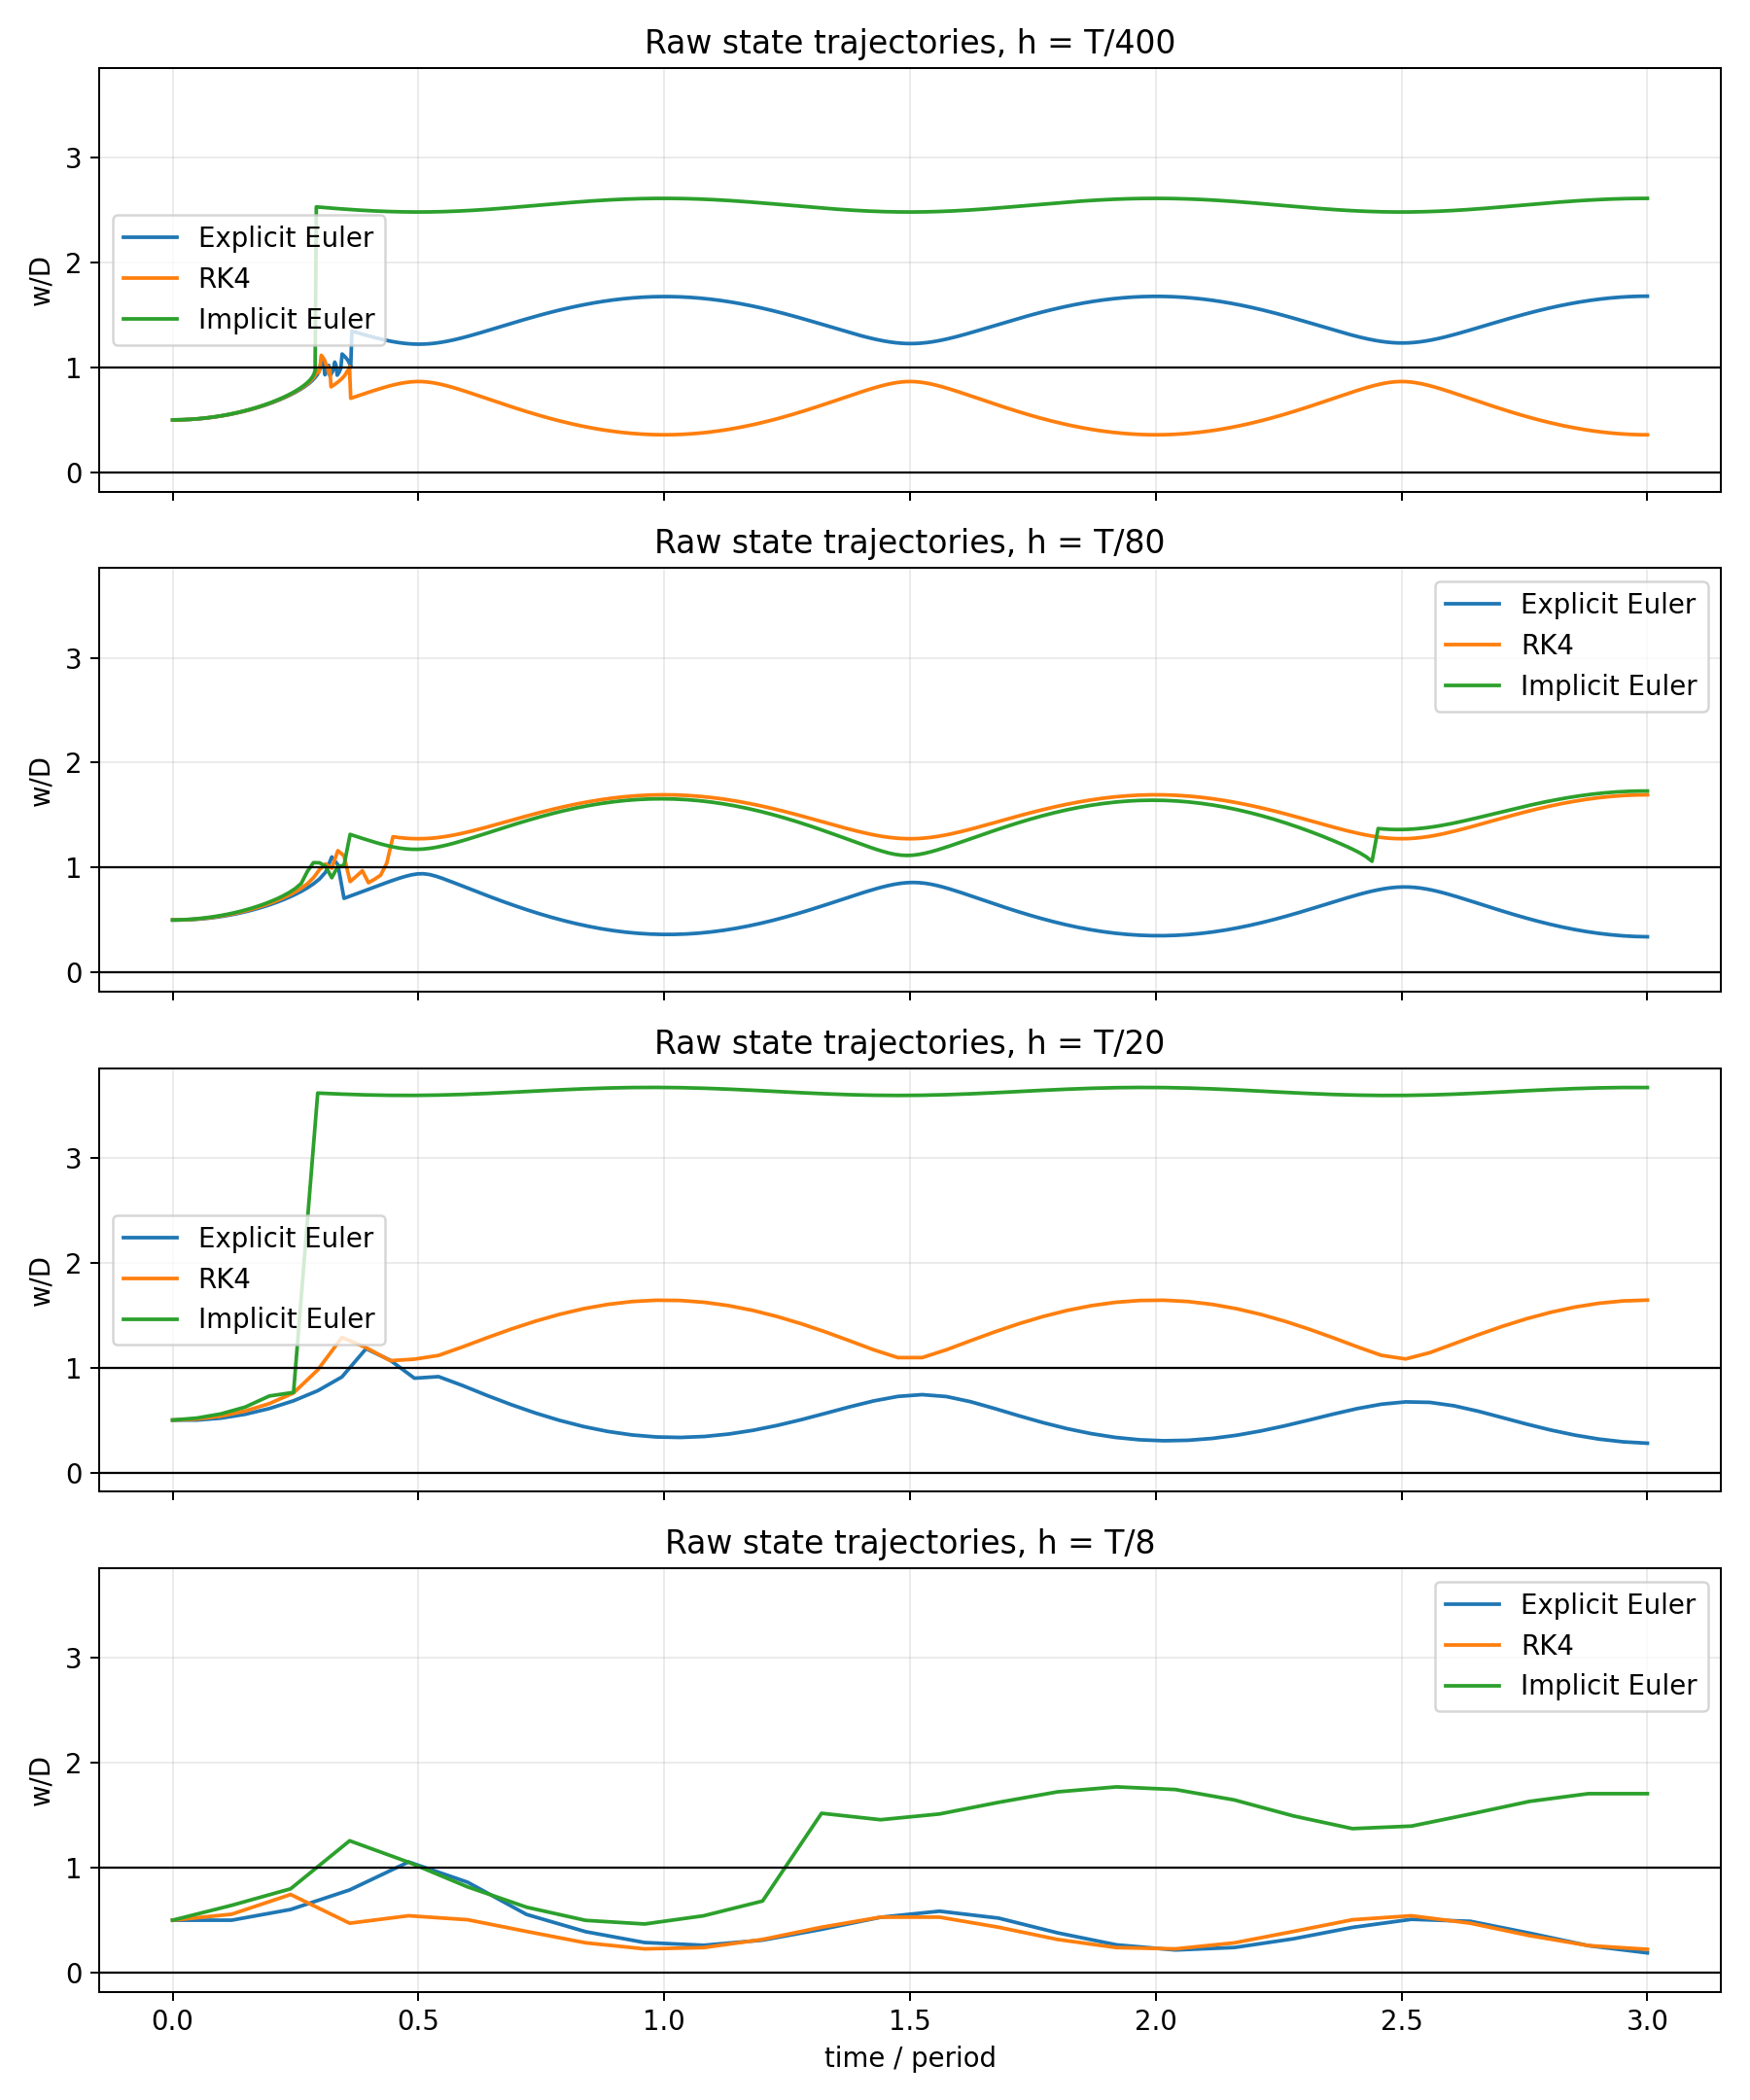
\includegraphics[width=\linewidth]{../figures/state_trajectories.png}
  \caption{Raw normalized state trajectories for all methods and step sizes.}
  \label{fig:state}
\end{figure}

The two most important reference levels are:
\[
w/D = 0,\qquad w/D = 1.
\]
The physically valid region is between these two lines. Any curve above \(1\) or below \(0\) is a raw numerical result that violates the physical state constraint.

The step-size labels are also important. \(T/400\) means the period is divided into 400 steps, so it is the finest timestep in the plot. \(T/8\) means only 8 steps per period, so it is the coarsest. A common mistake is to read a larger denominator as a larger timestep; here it is the opposite.

\subsection{Presentation explanation for Figure 1}

When presenting this figure, explain it as follows:
\begin{quote}
The plot shows the internal state of the memristor. A value of 0 means the doped region has zero width, and a value of 1 means it fills the device. The physical solution should stay between 0 and 1. We deliberately keep raw numerical values so we can see when a method overshoots. The different panels show different time steps. \(T/400\) is fine, while \(T/8\) is coarse. A coarse curve that appears bounded is not automatically more accurate, because it may simply be skipping important parts of the motion.
\end{quote}

\subsection{Interpretation of the state trajectories}

The state trajectories show that step size strongly affects the raw solution, but the trend is not monotone. In other words, increasing the timestep does not always create a visibly larger overshoot. A very coarse method can sometimes look better than an intermediate method because it under-samples the sinusoidal voltage and misses the portions of the cycle where the state would move strongly.

This explains a pattern that may look confusing during presentation: RK4 can look reasonable for \(T/400\), overshoot for \(T/80\) or \(T/20\), and then appear bounded again for \(T/8\). This does not mean the coarsest RK4 case is the best case. It means the coarse grid is too sparse to reliably resolve the dynamics. The absence of overshoot in a coarse raw trajectory is not the same thing as accuracy.

Even higher-order or implicit methods can leave the physical interval in this stress-case setup. This is not a contradiction. RK4 improves local accuracy for smooth problems, and Implicit Euler can improve stability for certain modes, but neither method automatically knows that \(w\) is a physical length unless the algorithm includes bound enforcement.

\subsection{Why the timestep trend is not clean}

There are two main reasons why the raw trajectories do not follow a simple coarse-step trend.

First, the applied voltage is sinusoidal. If the timestep is too coarse, the method samples only a few points on the sine wave. It may miss the peak or miss the interval where the state derivative is large. This is similar to taking too few photographs of a moving object: the object may appear to move less simply because the camera missed the motion.

Second, the raw memristor equation is not bound-preserving. It does not contain a mechanism that forces \(w\) to stop at \(0\) or \(D\). With the default parameters, the linear memristance formula approaches zero shortly above \(w/D=1\). Once a raw trajectory crosses the physical upper bound, the denominator in
\[
\frac{dw}{dt}
=
\frac{\mu_v R_{\text{on}} v(t)}{D^2 M(w)}
\]
can become very small. Small numerical differences can then cause large jumps in the next update. This makes the raw plot a stress test of unconstrained numerical updates, not a smooth ranking of methods.

\subsection{Does coarse RK4 being bounded mean coarse RK4 is good?}

No. A bounded-looking coarse RK4 trajectory should be treated with caution. It might be bounded because the method missed the part of the cycle that would have caused large movement. A simulation should be judged by both resolution and physical validity. If a method is too coarse to capture the forcing, it can look stable while being inaccurate.

\subsection{How to read the boundary violation plot}

Figure~\ref{fig:bounds} compresses the overshoot information into a bar chart. The vertical axis is the maximum violation normalized by \(D\). A value of zero means the raw trajectory stayed within the physical interval for that method and step size. However, this should be interpreted together with the state trajectory plot. A small violation can mean the method behaved well, but it can also mean the method was too coarse to see the movement.

\begin{figure}[H]
  \centering
  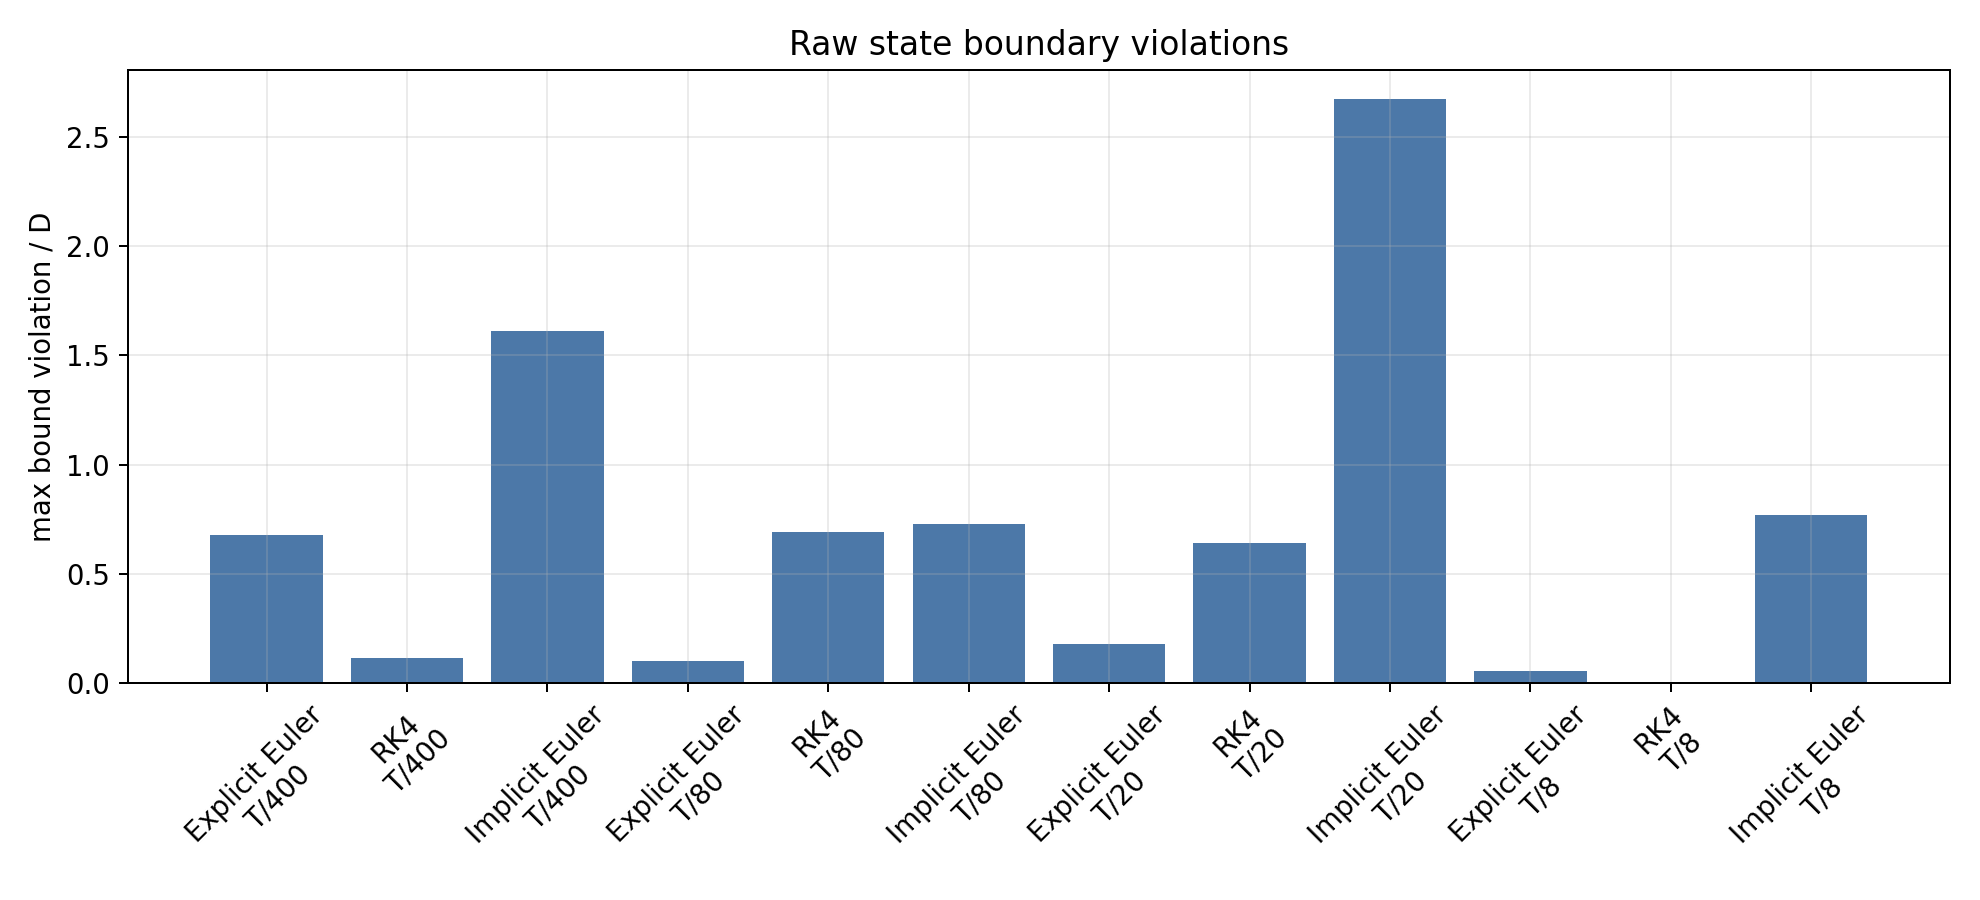
\includegraphics[width=\linewidth]{../figures/bound_violations.png}
  \caption{Maximum raw state boundary violation normalized by device thickness.}
  \label{fig:bounds}
\end{figure}

\subsection{Presentation explanation for Figure 2}

For presentation, this figure should be described as the direct physical-validity check:
\begin{quote}
This bar chart answers a simple question: how far did the raw computed state leave the physically allowed interval? A zero-height bar means no overshoot was observed. A taller bar means the numerical state became more physically unrealistic. But a zero-height or small bar is not automatically proof of accuracy, especially for coarse timesteps. This plot is important because it separates numerical smoothness from physical validity, but it should be read together with the timestep resolution.
\end{quote}

\subsection{Interpretation of the boundary violations}

The boundary plot confirms that the methods do not behave identically. Explicit Euler is simple and step-size dependent. RK4 can reduce error when the solution remains smooth and sufficiently resolved, but it can still overshoot under stress. Implicit Euler solves a future-time equation, but it is still solving the unbounded mathematical update; therefore, it can also leave the physical interval.

The boundary plot should not be used by itself to declare a winner. For example, Explicit Euler may have low cost and may show smaller overshoot in a particular coarse case, but it remains a first-order method. It can be cheap and still inaccurate. Similarly, RK4 can have a zero or small violation in a coarse case, but that may reflect missed dynamics rather than superior behavior.

\subsection{How to read the V-I hysteresis plot}

Figure~\ref{fig:hysteresis} plots current against voltage. Voltage is on the horizontal axis. Current is on the vertical axis. Because the voltage is sinusoidal, the system repeatedly moves forward and backward through voltage values.

\begin{figure}[H]
  \centering
  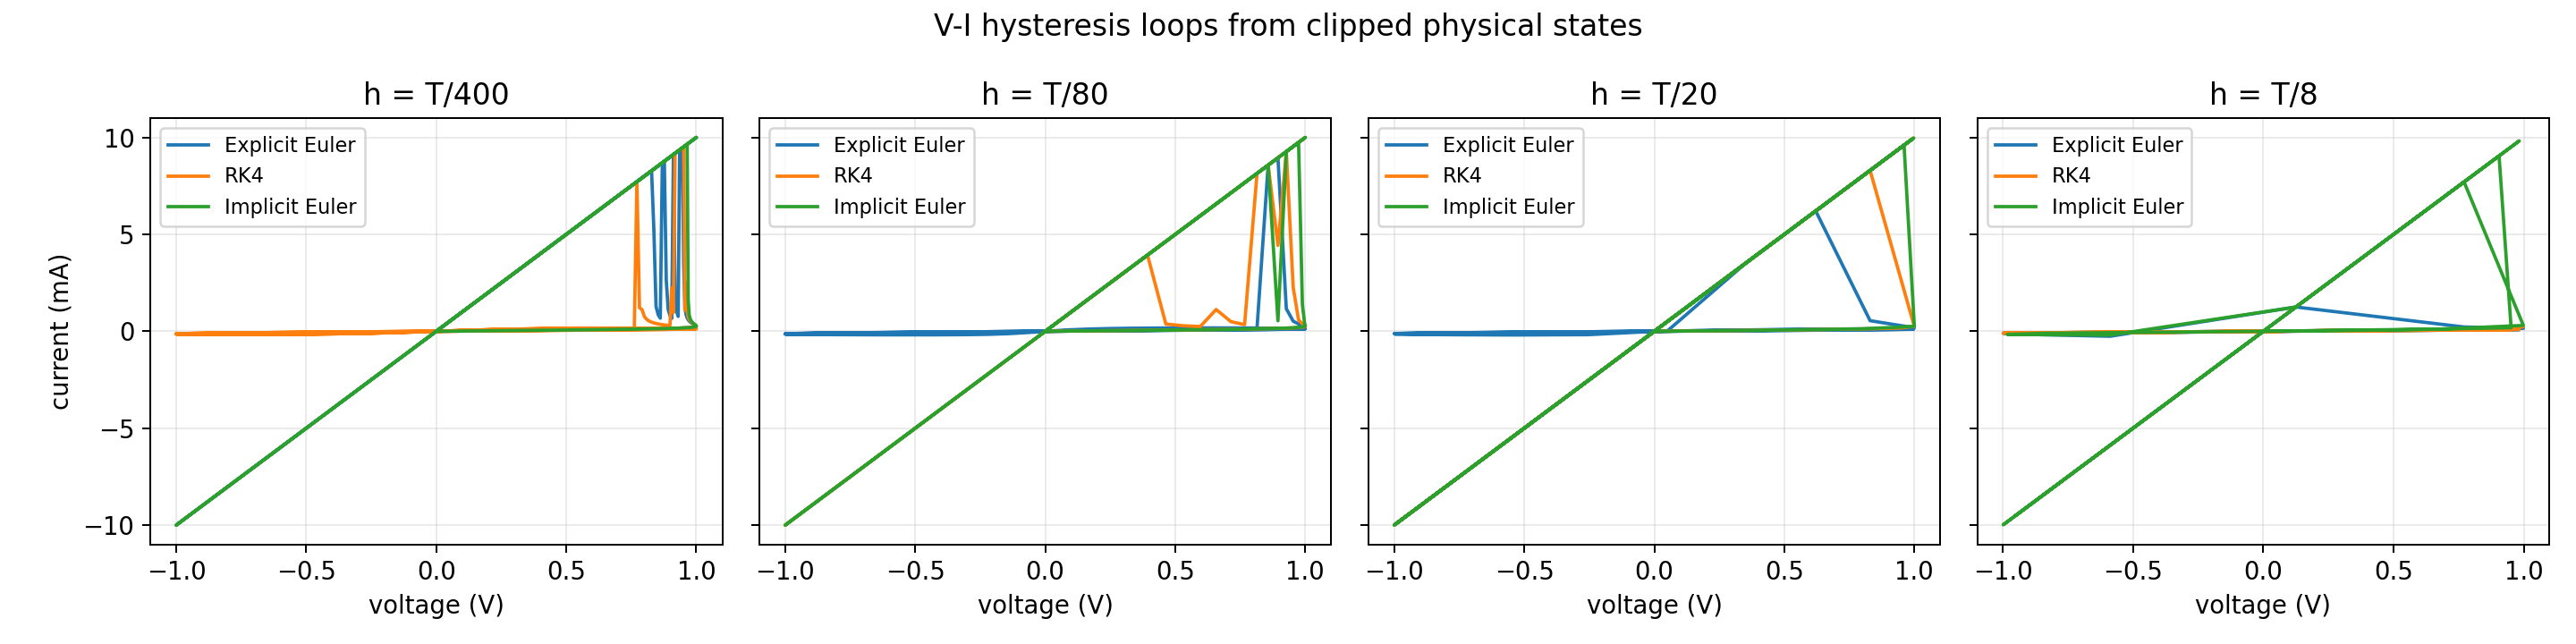
\includegraphics[width=\linewidth]{../figures/hysteresis_loops.png}
  \caption{Voltage-current hysteresis loops computed from clipped physical states.}
  \label{fig:hysteresis}
\end{figure}

If the device were a fixed resistor, the V-I curve would be a straight line. A loop indicates memory: the current at a given voltage can differ depending on whether the voltage is increasing or decreasing and depending on the internal state history.

\subsection{Why clipping is used for V-I curves}

The hysteresis plot uses clipped states because current is computed from memristance, and memristance is only physically meaningful when \(w\) is within the device. This does not erase the overshoot analysis, because overshoot is already measured using raw states in the previous figures and tables. The purpose of clipping here is to show the physically interpretable V-I response.

\subsection{Presentation explanation for Figure 3}

For presentation, use this explanation:
\begin{quote}
The V-I plot shows the device's memory effect. Instead of getting a single straight line like an ordinary resistor, we get loops because the resistance changes with the internal state. The loops are computed from clipped states, meaning we force the state into the physical interval only for this visualization. The raw overshoot is still shown separately in the state and boundary plots.
\end{quote}

\subsection{Interpretation of the hysteresis loops}

The V-I loops show how numerical differences in \(w(t)\) influence the observable electrical behavior. Methods and step sizes that produce different clipped state histories can produce different loop shapes. This is important because in experiments and applications, the current-voltage relationship is often the visible output, while the internal state is hidden.

For presentation, it is useful to connect this plot back to the raw state plot. The V-I curves are produced from clipped states, so they show a physically valid electrical response after enforcing the state interval for visualization. They do not erase the fact that the raw solver may have overshot. Therefore, the hysteresis plot is best interpreted as the observable behavior after physical clipping, while the state and boundary plots diagnose the raw numerical method.

\subsection{How to read the runtime plot}

Figure~\ref{fig:runtime} shows median runtime per time step. The y-axis is measured in microseconds per step. This normalizes the cost so that methods with different numbers of total steps can be compared fairly.

\begin{figure}[H]
  \centering
  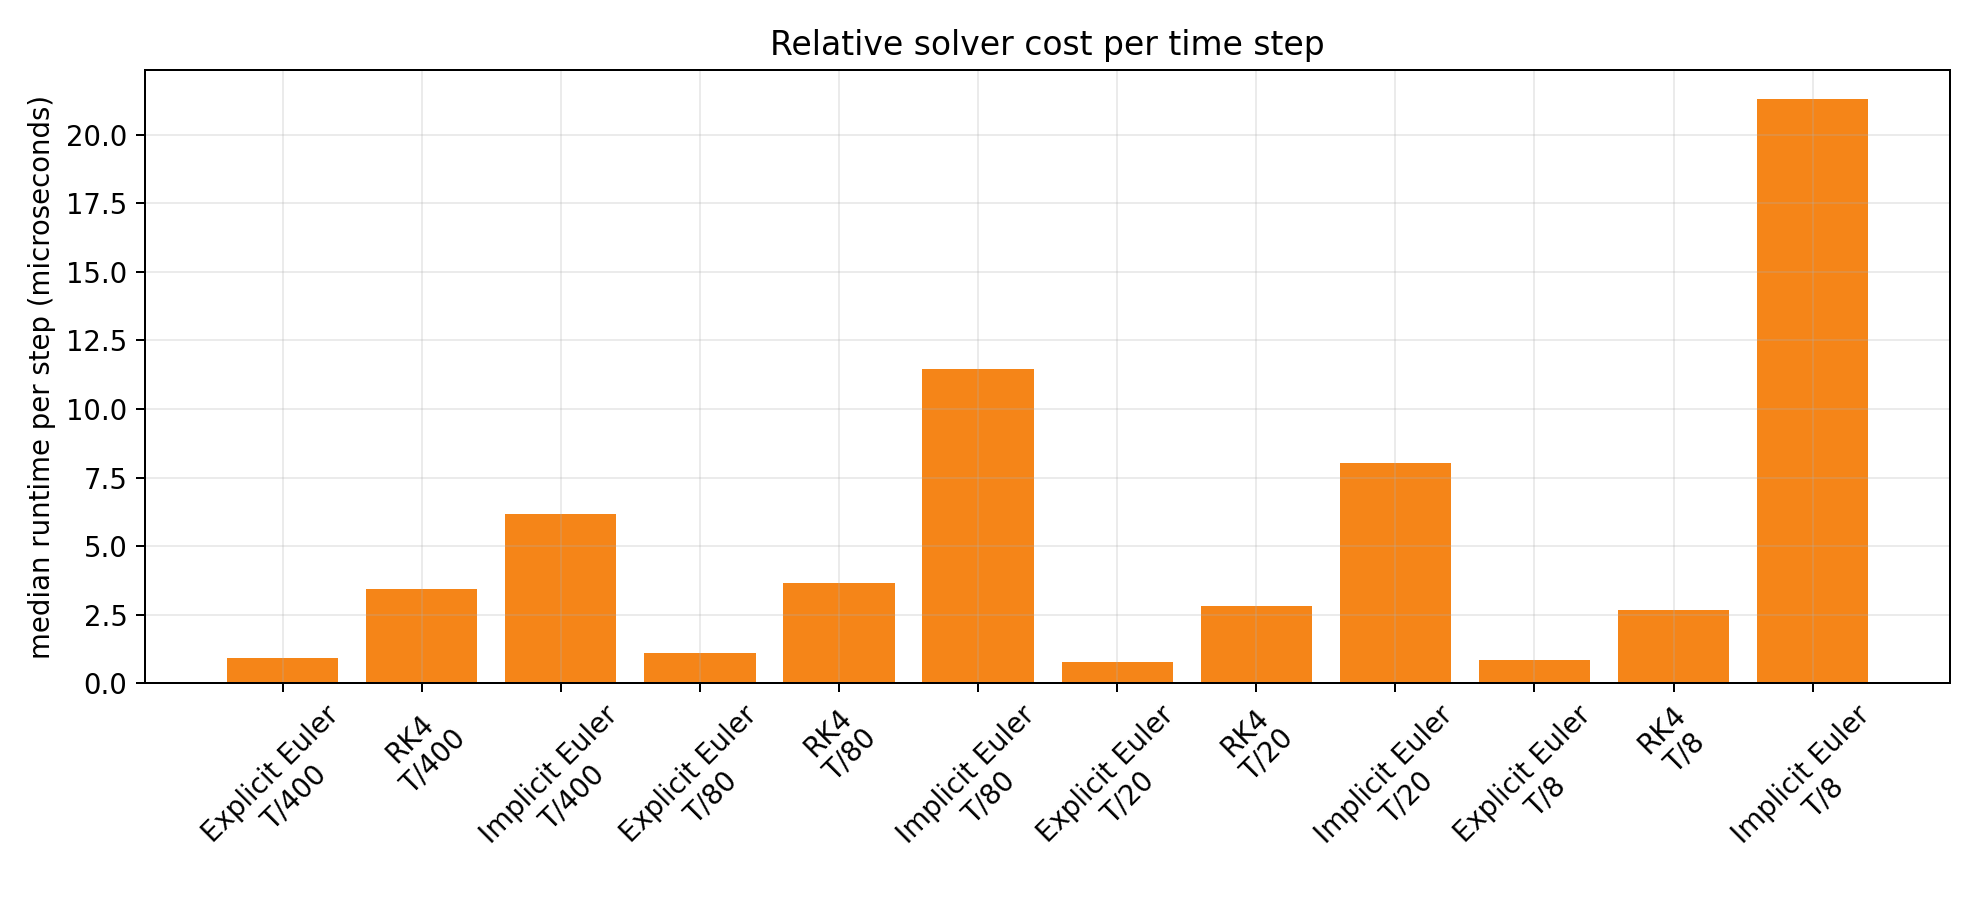
\includegraphics[width=\linewidth]{../figures/runtime_per_step.png}
  \caption{Median runtime per step over repeated solver calls.}
  \label{fig:runtime}
\end{figure}

\subsection{Presentation explanation for Figure 4}

For presentation, explain runtime as a secondary metric:
\begin{quote}
This plot compares computational cost per step. Explicit Euler is cheapest because it evaluates the derivative once. RK4 is more expensive because it evaluates four slopes per step. Implicit Euler is usually more expensive because it solves a nonlinear equation at each step. We should not overinterpret the exact numbers, but the relative cost pattern is useful. Cost is not enough to choose the best method: the cheapest method can still be inaccurate or physically invalid.
\end{quote}

\subsection{Does Explicit Euler beat the other methods because it is cheap?}

No. Explicit Euler is the cheapest method per step, but runtime is only one metric. A method must also resolve the dynamics and preserve or at least reveal physical validity. Explicit Euler uses only one slope at the start of each step, so it is first-order accurate and strongly dependent on timestep. Its lower runtime is useful, but it does not compensate for under-resolution or incorrect state evolution.

The correct presentation statement is: Explicit Euler is the cheapest baseline, RK4 is the stronger explicit accuracy baseline when the timestep is fine enough, and Implicit Euler demonstrates the cost and behavior of solving a future-time update. None of the raw methods alone is a complete physical memristor simulator because none enforces \(0 \leq w \leq D\) during the update.

\subsection{What should be concluded about timestep choice?}

The safe conclusion is not ``always use the lowest number of steps'' or ``always use the highest number of steps.'' The correct conclusion is that the timestep must be fine enough to resolve the forcing and the state movement. In this notation, \(T/400\) is finer than \(T/8\). A fine timestep is generally more trustworthy for resolving the ODE, but if the underlying raw model allows unphysical states, even a fine method can accurately follow the unbounded mathematical equation into an unphysical region.

Therefore, a physically reliable simulation needs two things:
\begin{itemize}[noitemsep]
  \item sufficient timestep resolution,
  \item a bound treatment, such as clipping, projection, or a model modification like a window function.
\end{itemize}

\section{Method-by-Method Discussion}

\subsection{Explicit Euler}

Explicit Euler is useful as a baseline because it is simple and transparent. It has low computational cost, but it is only first-order accurate. It is also sensitive to step size. In this project, that sensitivity matters because the state is physically bounded.

The main lesson from Explicit Euler is that a method can be easy to implement but fragile under time discretization. If it looks good in a coarse case, that result must still be checked against resolution and physical validity. Cheap runtime alone is not enough to make it the best method.

\subsection{RK4}

RK4 is a higher-order explicit method. It is generally much more accurate than Explicit Euler when the step size is sufficiently small and the trajectory is smooth. However, RK4 still does not enforce \(0 \leq w \leq D\). It can reduce numerical error, but it does not automatically solve the physical boundary problem.

The main lesson from RK4 is that higher accuracy is not the same as physical constraint preservation.

\subsection{Implicit Euler}

Implicit Euler uses future-time information. This often improves stability for certain decaying or stiff problems. In this project, however, the method still solves an unbounded equation unless additional constraint handling is added. The raw implicit trajectory can therefore overshoot.

The main lesson from Implicit Euler is that implicitness can help with stability, but it does not replace physical modeling decisions.

In this project, Implicit Euler can look poor in the raw trajectories because it is still solving the unbounded state equation. Its nonlinear solve can follow the implicit update into the unphysical region unless a bound constraint is added. This is why the result should be described carefully: Implicit Euler has useful stability properties in many IVPs, but those properties do not automatically make it bound-preserving for this memristor model.

\section{Important Distinctions}

\subsection{Accuracy versus stability}

Accuracy asks whether a method is close to the true solution. Stability asks whether errors grow uncontrollably. A method can be accurate for small steps but unstable or physically invalid for large steps. The project compares both behavior and physical validity.

\subsection{Numerical validity versus physical validity}

A numerical method can produce a finite number without producing a physically meaningful state. In this project, any raw state outside \([0,D]\) is physically invalid. This is why the boundary violation plot is essential.

\subsection{Apparent stability versus true resolution}

An apparently stable coarse curve can be misleading. If a method takes too few samples per period, it can miss peaks and rapid changes. This can make the output look calm even when it is not accurately representing the ODE. For this project, this distinction is central to explaining why the \(T/8\) RK4 case can appear better than some less coarse cases.

\subsection{Raw result versus clipped result}

The raw result tells us what the method actually computed. The clipped result tells us what current would look like if the state were forced back into the physical range. Both are useful, but they answer different questions.

\section{Limitations}

\subsection{Simplified memristor model}

The model used here is the linear ion drift HP TiO2 model. Real memristors can have more complicated nonlinear drift, threshold effects, window functions, temperature effects, and device variability. This project focuses on a simple model because the goal is numerical-method comparison.

\subsection{No adaptive step size}

The notebook uses fixed step sizes. Adaptive solvers can change step size automatically based on error estimates. They are not used here because the project aims to implement and compare the course-level methods directly.

\subsection{No built-in bound-preserving solver}

The project detects and measures boundary violations, but the raw methods are not modified to enforce bounds during each update. This is intentional because the proposal asks to compare overshoot behavior. A future extension could add bound-preserving variants.

\subsection{Runtime is environment-dependent}

Runtime measurements depend on hardware, Python overhead, and system load. They are useful for relative comparison within this notebook but should not be treated as universal benchmark values.

\section{Conclusion}

\subsection{Main conclusion}

The project shows that solving a memristor ODE is not only about producing a curve. The computed internal state must also remain physically meaningful. Explicit Euler, RK4, and Implicit Euler differ in accuracy, cost, and stability behavior, but none of them automatically enforces the physical bound \(0 \leq w \leq D\).

\subsection{What the plots collectively show}

The state trajectory plot shows the raw evolution of the internal state. The boundary violation plot directly identifies unphysical overshoot. The V-I hysteresis plot shows how the state affects observable electrical behavior after clipping for physical interpretation. The runtime plot shows the computational cost tradeoff. Together, the figures support the central message: method choice, step-size resolution, and boundary handling all matter.

The most important plot-analysis point is that the results are not a simple competition where the lowest-cost method wins or where the coarsest bounded-looking line is best. Coarse timesteps can hide dynamics, and the raw equation can leave the physical interval. The plots should therefore be presented as evidence for why bounded physical IVPs need both numerical resolution and physical constraint handling.

\subsection{Final presentation takeaway}

For a presentation, the clean takeaway is:
\begin{quote}
The memristor has memory because its resistance depends on an internal state. Numerically solving that state equation requires care. A method can look reasonable because it is coarse, cheap, or visually smooth, but still produce impossible internal states or miss important dynamics. Therefore, when simulating bounded physical systems, we must compare not only accuracy and runtime, but also timestep resolution and whether the numerical method respects physical constraints.
\end{quote}

\end{document}
